\subsection
{\href{http://cst.mi.fu-berlin.de/intern/19606-P-MPP/Aufgaben/040202.html}
{Aufgabe 6: Stromverbrauch und Taktfrequenz}}

Folgende Tabelle zeigt die Abhängigkeit des Stromverbrauchs von der Taktfrequenz. Der DCO\-CLK-Taktgenerator wurde durch manuelle Modifikation der DCOCTL, BCSCTL1 und BCSCTL2 Register im Debug-Modus des Code Composers auf Frequenzen im Bereich von 100kHz bis 10MHz eingestellt. Anschließend wurde jeweils der Stromverbrauch des Controllers im RUN-Modus am in Reihe geschalteten Digitalmultimeter gemessen. Die Tabelle enthält alle Messwerte mit den entsprechenden Bit-Settings der Clock-Register.

\begin{center}
\begin{tabular}{|r|c|c|c|c|c|}\hline
Frequenz in kHz	&	Strom in mA	&	RSEL	&	DCO	&	MOD	&	DIVM \\\hline

99,7	&	0,53	&	0	&	0	&	0	&	3 \\\hline
138,4	&	0,57	&	1	&	0	&	0	&	3 \\\hline
196,6	&	0,62	&	2	&	0	&	0	&	3 \\\hline
290,6	&	0,71	&	3	&	0	&	0	&	3 \\\hline
393,7	&	0,81	&	4	&	0	&	0	&	3 \\\hline
505,3	&	0,91	&	5	&	0	&	0	&	3 \\\hline
589,3	&	0,99	&	6	&	0	&	0	&	3 \\\hline
666,1	&	1,06	&	7	&	0	&	0	&	3 \\\hline
986,3	&	1,34	&	7	&	4	&	0	&	3 \\\hline
1.458,0	&	1,75	&	7	&	7	&	0	&	3 \\\hline
1.971,0	&	1,87	&	7	&	4	&	0	&	2 \\\hline
2.916,0	&	2,53	&	7	&	7	&	0	&	2 \\\hline
3.940,0	&	2,91	&	7	&	4	&	0	&	1 \\\hline
4.096,0	&	3,02	&	7	&	4	&	11	&	1 \\\hline
5.827,0	&	4,05	&	7	&	7	&	0	&	1 \\\hline
7.368,0	&	4,67	&	5	&	5	&	29	&	0 \\\hline
7.870,0	&	4,94	&	7	&	4	&	0	&	0 \\\hline
11.612,0	&	6,88	&	7	&	7	&	0	&	0 \\\hline

\end{tabular}
\end{center}

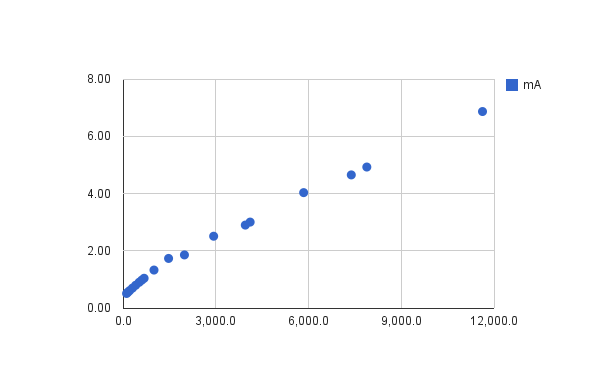
\includegraphics[width=\textwidth]{aufgaben/06/chart_2.png}

Das Diagramm zeigt den Stromverbrauch (vertikal) im Verhältnis zur Taktfrequenz (horizontal) der MCLK an Hand obiger Messwerte. Der Stromverbrauch stieg bei unseren Messungen grob proportional zur Taktfrequenz.

